\section{Classification pipeline}
Data on the Internet is sometimes questionable. We can use classification to assess the credibility of information found on the web.

\begin{figure}[!ht]
  \centering
  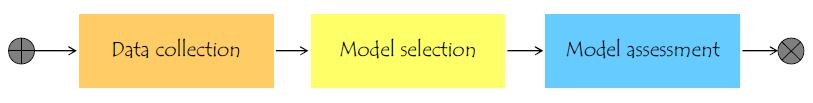
\includegraphics[width=0.8\linewidth]{figures/classification_pipeline}
  \caption{Classification pipeline}
  \label{fig:classificationPipeline}
\end{figure}

\subsection*{Data collection}
Definition of the attributes that describe a data item and the class label. Domain knowledge is needed to know which attributes are relevant for the classification task.

As shown on Figure \ref{fig:dataCollection}, here a the different step in our data collection pipeline:
\begin{enumerate}
	\item Definition of the features that describe a data item
	\item Label the data items to create a training set
	\item Discretisation of the features
	\item Selection of the relevant features
	\item Normalisation of the features
\end{enumerate}

\begin{figure}[!ht]
  \centering
  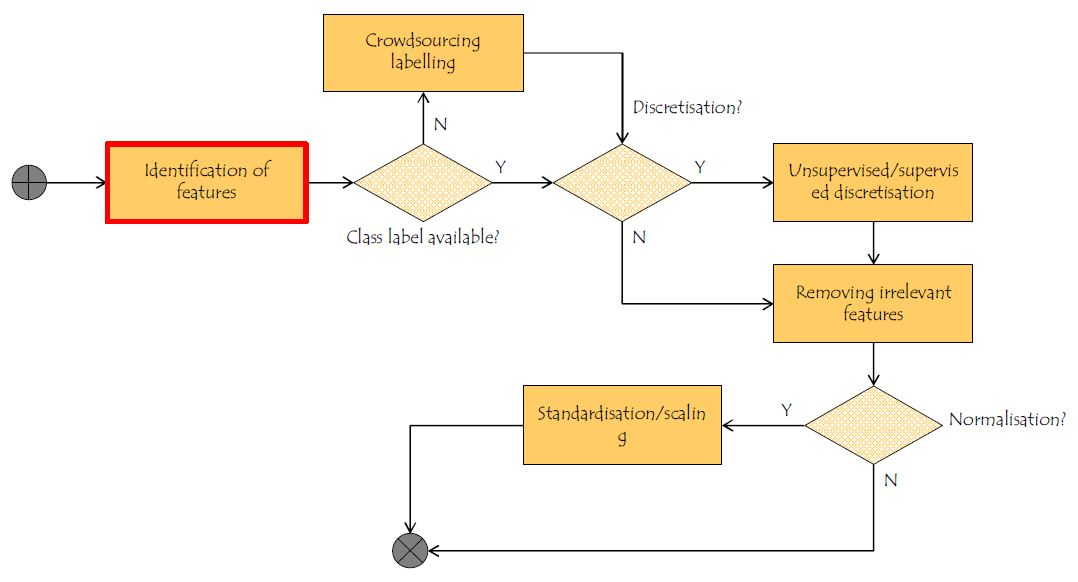
\includegraphics[width=0.8\linewidth]{figures/data_collection}
  \caption{Data collection pipeline}
  \label{fig:dataCollection}
\end{figure}
There exist different types of features:
\begin{itemize}
	\item Numerical (e.g., age, temperature)
	\item Ordinal (e.g., phone code, ...)
	\item Categorical (e.g., student, animals, ...)
\end{itemize}

It is easy to collect data on the web but difficult to label them. The basic idea of crowdsourcing is to enroll a large group of people that will contribute to a specific task. It suits really well for labelling a large data set. However, some of the workers aren't truthful, reliable, and are even sometimes random.

\subsubsection*{Aggregation algorithms}
Given the labelling provided by workers, requester might face the problem of aggregating the answers when they don't coincide.

There are two main classes of aggregation algorithms:
\begin{itemize}
	\item \textbf{Non-iterative}: take the matrix of answers provided by the workers, pre-process it and produce an estimate of the probability that a webpage X is labelled by label L.

	\textbf{Majority decision} algorithm is fast and appropriate for on-line aggregations but very sensitive to spammers. It estimates $P(x_j = l)$ as 
	\begin{align*}
		P(x_j = l) = \frac{1}{N} \sum_{i = 1}^N (1 | a_i(x_j) = j)
	\end{align*}
	with $x_j$ the webpage, $N$ the number of workers, $l$ le label and $a_i(x_j)$ the answer of worker $i$.

	\item \textbf{Iterative}: take the matrix of answers provided by the worker and produce an estimate of the probability that a webpage X is labelled by label L. With this estimate they update the \textbf{expertise of each worker}, that is, a metric that indicates how good is the worker at performing the labelling task. With this new information, the probability that a webpage X is labelled by label L is estimated again. This cycle continues until convergence.
\end{itemize}